\documentclass[conference]{IEEEtran}

\usepackage{amsmath,amssymb}
\usepackage{booktabs}
\usepackage{graphicx}
\usepackage{array}
\usepackage{multirow}
\usepackage{cite}
\usepackage{url}
\usepackage[hidelinks]{hyperref}

\graphicspath{{figures/}}

\newcommand{\ProtoH}{ProtoHedge}
\newcommand{\DeepH}{Deep Hedging}
\newcommand{\OCE}{\mathrm{OCE}}
\newcommand{\CVaR}{\mathrm{CVaR}}
\newcommand{\Offset}{\mathcal{O}}

\begin{document}

\title{ProtoHedge Beyond Simulation: An Audited Historical Evaluation of Interpretable Deep Hedging}

\author{
\IEEEauthorblockN{Yanis Zaim\IEEEauthorrefmark{1}, Sayak Chakrabarty\IEEEauthorrefmark{2}, and Imon Banerjee\IEEEauthorrefmark{2}}
\IEEEauthorblockA{\IEEEauthorrefmark{1}Columbia University, New York, NY, USA\\
Email: ymz2108@columbia.edu}
\IEEEauthorblockA{\IEEEauthorrefmark{2}Northwestern University, Evanston, IL, USA\\
Emails: sayak.chakrabarty@northwestern.edu, imon.banerjee@northwestern.edu}
}

\maketitle

\begin{abstract}
Deep Hedging learns sequential hedging decisions directly from market states,
frictions, and a risk-sensitive objective, but its neural policies are difficult
to inspect. ProtoHedge replaces the final black-box action map with a similarity-
weighted dictionary of representative market states. The original study found
that this bottleneck was nearly as effective as Deep Hedging in synthetic
Black--Scholes and stochastic-volatility environments. We ask whether that
conclusion survives historical option data and a path-dependent liability.
First, using frozen snapshots of the released TensorFlow source, we reproduce
the original ordering: ProtoHedge minus Deep Hedging optimized-certainty-
equivalent CVaR@50\% utility is $-9.10\times10^{-4}$ in the executed
Black--Scholes notebook configuration and $-1.48\times10^{-4}$ under stochastic
volatility. We then construct 34,395 contract-consistent rolling episodes for
ten U.S. equities and exchange-traded funds, with chronological train,
validation, and 2022--2024 test periods, a fixed listed hedge option within
each episode, explicit costs, and bounded inventories. The historical study
tests European and arithmetic-average Asian short-call liabilities using three
seeds and a validation-selected expanded ProtoHedge family. A post-run audit
found that a diagnostic-penalized checkpoint score selected the initialized
Deep Hedging policy in 12 of 60 fits. A targeted sensitivity that replaces
those affected comparisons using pure validation OCE changes the European
conclusion from apparent superiority to near parity. Under this conservative
sensitivity, European intervals contain zero, while the Asian tail-selected
policy has a panel utility advantage of $0.004015$ with a 95\% paired
temporal-block interval $[0.001925,0.006038]$. A one-seed SPY sensitivity finds
no detectable difference between the historical PyTorch soft-clipping map and
the exact TensorFlow Probability map. Prototype assignments are non-uniform and
traceable to historical states. The evidence therefore supports synthetic and
historical European near parity, together with a promising path-dependent tail
result, but not universal ProtoHedge superiority or superiority over an equally
tuned Deep Hedging family.
\end{abstract}

\begin{IEEEkeywords}
deep hedging, ProtoHedge, interpretable machine learning, option hedging,
sequential decision making, conditional value-at-risk, empirical finance
\end{IEEEkeywords}

\section{Introduction}

Hedging is a sequential decision problem under uncertainty. At every trading
date, a hedger must act using incomplete state information, absorb transaction
costs, respect position constraints, and manage a terminal loss distribution
rather than only an expected outcome. Deep Hedging addresses this problem by
training a policy end-to-end against a monetary utility objective
\cite{buehler2019deep}. This flexibility is useful when rebalancing is discrete,
frictions matter, or market dynamics are too complex for a closed-form hedge.
It also creates a practical problem: the resulting action is the output of a
neural network whose economic rationale can be difficult to audit.

ProtoHedge (\ProtoH) was introduced as an interpretable alternative
\cite{faloughi2025protohedge}. It represents a decision as a convex combination
of actions attached to a finite library of representative states, or
prototypes. The policy still learns from the same risk-sensitive objective, but
its action can be traced to a small set of examples. The original experiments
reported near parity with a standard Deep Hedging (\DeepH) network in
Black--Scholes and stochastic-volatility simulators. That finding is valuable,
but it leaves two questions open. First, does the released implementation
reproduce the reported synthetic model ordering when its exact utility metric
and stored artifacts are used? Second, does the performance--interpretability
tradeoff survive historical listed-option paths, changing market regimes, and
a path-dependent payoff?

These are not merely requests for a larger benchmark. Historical evaluation
changes the scientific problem. Listed contracts have finite lives and cannot
be replaced each day without implicitly rolling the hedge. Nearby rolling
episodes are strongly dependent. A chronological split is needed to prevent
future leakage. The current inventory, rather than only the latest trade, must
accrue one-step gains. An Asian payoff additionally requires an observable
running-average state. Finally, validation and checkpoint rules become part of
the estimand: a policy chosen by a diagnostic-penalized score is not the same
policy as one chosen by the paper's utility.

We address these issues in a sequence of linked experiments, summarized in
Fig.~\ref{fig:study-design}. We first execute the released TensorFlow model from
frozen source snapshots in the two synthetic environments. We then evaluate a
PyTorch historical implementation on 34,395 contract-consistent 20-decision
episodes spanning ten liquid equities and exchange-traded funds. The test
calendar is 2022--2024. All candidate selection is performed on the training
and validation periods. We compare unhedged exposure, a market-delta rule, a
validation-tuned no-trade band, one fixed paper-style DH architecture, and a
validation-selected expanded PH family. We finally audit checkpoint semantics,
the scope of the expanded family, the PyTorch SoftClip approximation, and the
empirical prototype assignments.

\begin{figure*}[t]
\centering
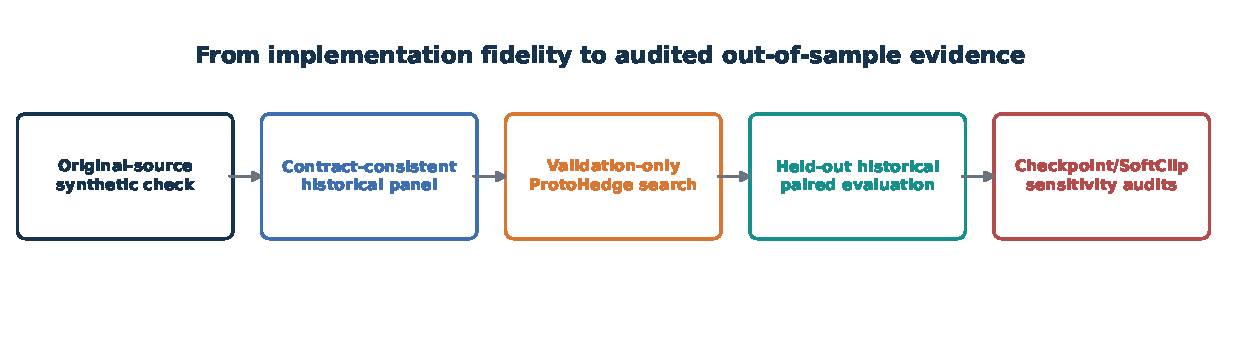
\includegraphics[width=0.98\textwidth]{study_design.pdf}
\caption{Evidence flow. Synthetic confirmation and the historical study answer
different questions and are not pooled. The final historical interpretation
incorporates targeted checkpoint and implementation-sensitivity audits.}
\label{fig:study-design}
\end{figure*}

The principal result is deliberately qualified. The original executed
historical checkpoint rule suggested a broad PH advantage, especially for
European calls. The audit showed that this result was partly attributable to
the benchmark checkpoint rule: 12 of 60 DH fits selected their initialized
state. Replacing the identified affected comparisons under pure validation OCE
reduced the European PH--DH utility gaps by 89--92\%, and both European
intervals then included zero. This near-parity result is consistent with the
original synthetic evidence rather than a failed outcome. For Asian calls, the
tail-selected PH result changed little and retained a positive panel interval.
Thus, the most defensible interpretation is that the prototype bottleneck
preserves performance on terminal-payoff historical tasks and may offer a tail
advantage when the liability is path dependent.

The paper makes five contributions:
\begin{enumerate}
    \item We provide a source-level reproduction of the original PH--DH
    comparison under Black--Scholes and stochastic-volatility dynamics, using
    the original OCE CVaR@50\% utility and documenting a material discrepancy
    between the Black--Scholes prose specification and executed notebook.
    \item We construct a leakage-resistant historical panel in which each
    episode follows one fixed listed option contract, contains 20 trade
    decisions and 21 marks, and lies wholly inside a chronological period.
    \item We extend the comparison to European and arithmetic-average Asian
    liabilities with common information, accounting, costs, bounds, and test
    paths.
    \item We use paired temporal-block inference and add direct comparisons
    with a transparent Spot-Delta baseline, rather than treating DH as the only
    benchmark.
    \item We audit checkpoint selection, model-family scope, action clipping,
    saturation, and prototype usage. The audit changes the headline European
    claim and is therefore part of the scientific result, not an implementation
    footnote.
\end{enumerate}

Our claim is correspondingly narrow. We do not claim that PH dominates DH on
every asset or metric, that the historical grid is an unchanged copy of the
released PH model, that the one-seed implementation sensitivity replaces a
panel experiment, or that the selected PH family beats a comparably tuned DH
family. We claim that (i) the original synthetic near-parity ordering can be
recovered from the released workflow, (ii) historical European performance is
consistent with near parity after a conservative checkpoint sensitivity, and
(iii) a validation-tail-selected expanded PH family exhibits a positive Asian
OCE CVaR@50\% panel result that merits further confirmation.

\section{Background and Related Work}

\subsection{Deep Hedging as Risk-Sensitive Sequential Control}

Let $P_t\in\mathbb{R}^{m}$ be the vector of hedge-instrument prices at decision
time $t$, $h_{t-1}$ the inventory carried into that decision, and $x_t$ the
observable state. A policy proposes a trade increment
\begin{equation}
    a_t=\pi_\theta(x_t), \qquad
    h_t=\Pi_{\mathcal H}(h_{t-1}+a_t),
    \label{eq:policy}
\end{equation}
where $\Pi_{\mathcal H}$ enforces the cumulative-position set. For terminal
short-liability cash flow $H\leq0$ and per-unit trading-cost vector $\kappa_t$,
the premium-excluding liability offset is
\begin{equation}
\Offset^\pi
=H+\sum_{t=0}^{T-1}h_t^\top(P_{t+1}-P_t)
-\sum_{t=0}^{T-1}\kappa_t^\top|a_t|.
\label{eq:offset}
\end{equation}
Higher $\Offset$ means that the hedge offsets more of the common short
liability after costs.

The learned objective is the optimized certainty equivalent used in the Deep
Hedging codebase:
\begin{equation}
\mathcal U_\lambda(\Offset)
=\sup_{y\in\mathbb R}\mathbb E\left[(1+\lambda)
\min(\Offset+y,0)-y\right].
\label{eq:oce}
\end{equation}
For the software's \texttt{cvar} utility, the associated lower-tail probability
is $p=(1+\lambda)^{-1}$. We set $\lambda=1$, hence $p=0.5$. The scalar threshold
$y$ is learned jointly with the policy. At evaluation we freeze each trained
model's threshold and average its pathwise utility contribution. We refer to
this quantity as \emph{frozen-threshold OCE CVaR@50\% utility}. It is the metric
used for the original-paper reproduction and the primary PH--DH comparison.
It is distinct from the separately calculated empirical lower-tail means at
50\% and 5\% \cite{rockafellar2000}.

A standard DH policy implements $\pi_\theta$ as a feed-forward neural network.
It is an essential benchmark because it can consume the same state, optimize
the same objective, and obey the same constraints as PH. Related work has
studied neural hedging under richer market dynamics \cite{gao2023deeper}; our
focus is narrower: the behavior of an interpretable prototype bottleneck under
historical data and explicit protocol audits.

\subsection{ProtoHedge}

Let $\mathcal P=\{p_1,\ldots,p_K\}$ be fixed representative states. For a
standardized state $\widetilde{x}_t$, nonnegative feature weights $\gamma$, and
a learned shared projection $f_\phi$, the historical PH implementation forms
\begin{align}
z_t &=f_\phi(\gamma\odot\widetilde{x}_t), &
z_k^p&=f_\phi(\gamma\odot p_k),\\
d_{t,k}&=\|z_t-z_k^p\|_2^2, &
\alpha_{t,k}&=\frac{\exp(-d_{t,k})}
{\sum_{j=1}^{K}\exp(-d_{t,j})}.
\label{eq:similarity}
\end{align}
Each prototype has a learned bounded action $b_k\in\mathbb R^m$, and
\begin{equation}
    a_t=\sum_{k=1}^{K}\alpha_{t,k}b_k.
    \label{eq:proto-action}
\end{equation}
Equation~\eqref{eq:proto-action} makes the local explanation exact with respect
to the model: the reported prototype weights and actions are the quantities
that generate the decision. This is stronger than attaching an explanation to
a separately trained black box, although it does not by itself prove that each
prototype has a stable economic interpretation.

The original PH motivation is a performance--interpretability tradeoff rather
than universal performance dominance \cite{faloughi2025protohedge}. Fixed
anchors preserve the connection between a prototype and an observed state;
the projection and prototype actions remain trainable. Our historical grid
retains this mechanism but expands the candidate family, as detailed in
Section~\ref{sec:models}.

\subsection{Why Historical Validation Is Different}

Simulation provides exact control over dynamics and can generate independent
paths. Historical option data instead combine non-stationarity, quote noise,
liquidity variation, market closures, overlapping trajectories, and a finite
set of listed contracts. A valid empirical test must therefore specify the
contract path, payoff state, temporal split, dependence-aware uncertainty, and
model selection process. These design choices are central to this study. They
also explain why the synthetic and historical numbers answer related but
non-interchangeable questions: the former tests implementation fidelity under
the original worlds; the latter tests out-of-sample behavior under observed
paths.

\section{Original-Source Synthetic Confirmation}
\label{sec:synthetic}

\subsection{Protocol}

We exported frozen snapshots of the released TensorFlow implementation rather
than substituting the PyTorch historical port. The Black--Scholes confirmation
uses source commit \texttt{983da37765b0}; the stochastic-volatility confirmation
uses the archived released source at \texttt{aedb45060622}. Both use TensorFlow
2.13, 20 steps of length $0.02$, 10,000 training paths, 1,000 validation paths,
800 epochs, Adam with learning rate $10^{-3}$, batch size 32, model seed 1, and
the OCE objective in Eq.~\eqref{eq:oce}. The DH network has width 20, depth 3,
and Softplus activations. PH uses $K=100$ for Black--Scholes and $K=500$ for
stochastic volatility, following the corresponding released notebook assets.
The paired deterministic test contains 10,000 Black--Scholes paths and 5,000
stochastic-volatility paths.

The checkpoint rule matches the original trainer: minimize training OCE over
the initialized checkpoint and 800 trained epochs. This rule is retained here
because the purpose is faithful reproduction. It should not be confused with
the chronological validation selection used for historical data.

\subsection{Black--Scholes Configuration Reconciliation}

The released materials contain a reproducibility ambiguity. The prose-level
paper configuration indicates zero drift and names a zero-drift, $K=100$
prototype file, but that file is absent from the released revisions. The
executed author notebook instead uses the simulator's default drift $0.1$ and
the committed $K=100$ prototype asset. We report both paths rather than hiding
the discrepancy. Regenerating the missing zero-drift prototypes produced a
PH--DH gap of $-0.008841$. Replaying the executed notebook configuration with
its committed prototypes reduced the gap to $-0.000910$, while the saved
notebook outputs imply $-0.000255$. Table~\ref{tab:bs-reconciliation} records
the reconciliation. The executed-notebook configuration is our headline
Black--Scholes confirmation because it is the closest reproducible account of
what generated the stored author results; the zero-drift attempt remains part
of the archive as a sensitivity.

\begin{table*}[t]
\centering
\footnotesize
\resizebox{0.94\textwidth}{!}{\begin{tabular}{lllrrr}
\toprule
Protocol & Drift & Prototype input & DH & PH & PH-DH \\
\midrule
Paper-specification attempt & 0.0 & regenerated K=100 & -0.058347 & -0.067188 & -0.008841 \\
Notebook-faithful confirmation & 0.1 & committed K=100 & -0.058102 & -0.059013 & -0.000910 \\
Saved author notebook & 0.1 & committed K=100 & -0.058166 & -0.058421 & -0.000255 \\
\bottomrule
\end{tabular}
}
\caption{Reconciliation of the released Black--Scholes specification and
executed notebook. Utility is frozen-threshold OCE CVaR@50\%; higher is better.
The missing zero-drift prototype input cannot be recovered exactly and was
regenerated in the first row.}
\label{tab:bs-reconciliation}
\end{table*}

\subsection{Synthetic Results}

Table~\ref{tab:synthetic-results} and Fig.~\ref{fig:synthetic-results} show the
confirmed results. PH is slightly below DH in both environments, reproducing
the direction reported in the original paper. The Black--Scholes gap is
$-0.000910$ versus the paper's approximately $-0.000230$; the
stochastic-volatility gap is $-0.000148$ versus approximately $-0.000300$.
Absolute Black--Scholes utility errors relative to the saved notebook are
$6.3\times10^{-5}$ for DH and $5.92\times10^{-4}$ for PH. Given stochastic
optimization and an unrecorded original test-clone seed, this is a sufficiently
close directional and scale confirmation for our purpose, but not bitwise
replication.

\begin{table}[t]
\centering
\footnotesize
\resizebox{\columnwidth}{!}{\begin{tabular}{lrrrr}
\toprule
Environment & Deep Hedging & ProtoHedge & PH-DH & Paper PH-DH \\
\midrule
Black--Scholes & -0.058102 & -0.059013 & -0.000910 & -0.000230 \\
Stochastic volatility & -0.090150 & -0.090299 & -0.000148 & -0.000300 \\
\bottomrule
\end{tabular}
}
\caption{Original-source synthetic confirmation. PH-DH is the difference in
frozen-threshold OCE CVaR@50\% utility; negative values favor DH. The final
column reports the approximate differences in the original PH paper.}
\label{tab:synthetic-results}
\end{table}

\begin{figure*}[t]
\centering
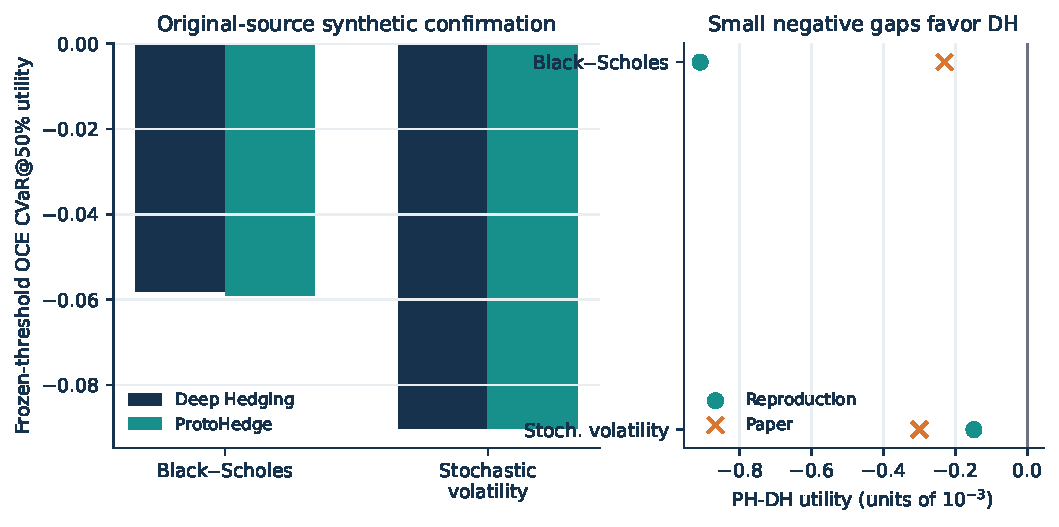
\includegraphics[width=0.88\textwidth]{synthetic_reproduction.pdf}
\caption{Synthetic utility levels (left) and PH--DH differences (right). Both
confirmations preserve the original ordering and near-parity interpretation.}
\label{fig:synthetic-results}
\end{figure*}

The Black--Scholes DH model has 943 trainable parameters and PH has 102, a
$9.25\times$ ratio. This compactness does not hold mechanically for every $K$:
the $K=500$ stochastic-volatility PH model has 1,359 parameters versus 1,004
for DH. Parameter efficiency is therefore configuration dependent, while the
prototype-based action decomposition remains present by construction.

\section{Historical Experimental Design}
\label{sec:historical-design}

\subsection{Data and Contract-Consistent Episodes}

We combine historical U.S. listed-option data from OptionMetrics IvyDB US with
daily underlying histories \cite{wrdsOptionMetrics,crspStock}. The final panel
contains AAPL, IWM, NVDA, QQQ, SPY, TLT, XLE, XLF, XLK, and XLV. The underlying
set spans single names, broad-market and sector equity funds, and a Treasury
fund. The available feature dates run from January 2005 through December 2024.

We retain American-style calls with finite implied volatility and vendor
Greeks, positive bids, non-crossed offers, positive midquotes, and positive
implied volatility. The listed option price is the bid--ask midpoint. At the
start of each candidate episode, eligible contracts have 20--40 calendar days
to expiration, initial open interest of at least one, relative spread at most
one, and absolute strike moneyness at most 10\%. Candidates are ranked by
absolute strike distance from spot, distance from a 30-day target maturity,
spread, open interest, and volume.

Most importantly, selection occurs once. An episode is retained only if the
same \texttt{optionid}, expiration, and strike have valid quotes at all 21
observations and the option expires after the episode. Thus, the listed option
is a genuine fixed hedge instrument rather than a daily sequence of unrelated
near-ATM contracts. A new contiguous block begins after any gap longer than
four calendar days.

The calendar is split before rolling windows are constructed. Training ends on
December 31, 2018; validation spans 2019--2021; and test spans 2022--2024. A
20-observation embargo is removed at each post-training boundary. No episode
crosses a period, although adjacent episodes within a period can overlap. The
corrected panel contains 34,395 episodes: 20,537 training, 6,881 validation,
and 6,977 test episodes. Counts by ticker appear in Table~\ref{tab:episode-counts}.

\begin{table*}[t]
\centering
\small
\begin{tabular}{lrrrr}
\toprule
Ticker & Train & Validation & Test & Total \\
\midrule
AAPL & 2,081 & 686 & 711 & 3,478 \\
IWM & 2,352 & 696 & 713 & 3,761 \\
NVDA & 1,775 & 666 & 644 & 3,085 \\
QQQ & 2,350 & 713 & 692 & 3,755 \\
SPY & 2,390 & 716 & 713 & 3,819 \\
TLT & 2,026 & 706 & 712 & 3,444 \\
XLE & 2,214 & 640 & 710 & 3,564 \\
XLF & 1,939 & 682 & 705 & 3,326 \\
XLK & 1,643 & 697 & 697 & 3,037 \\
XLV & 1,767 & 679 & 680 & 3,126 \\
Total & 20,537 & 6,881 & 6,977 & 34,395 \\
\bottomrule
\end{tabular}

\caption{Contract-consistent historical episodes. Each row contains 20
decision intervals and 21 observations. Windows may overlap within a period
but cannot cross the chronological split or embargo.}
\label{tab:episode-counts}
\end{table*}

The raw feature tensor at each observation is
\begin{equation}
x_t^{\mathrm{raw}}=(S_t,C_t,\Delta_t^{\mathrm{call}},
\nu_t,\sigma_t^{\mathrm{impl}}),
\end{equation}
where $C_t$ is the fixed listed call midpoint, $\Delta_t^{\mathrm{call}}$ and
$\nu_t$ are its vendor delta and vega, and $\sigma_t^{\mathrm{impl}}$ is its
implied volatility. Spot, option price, and vega are divided pathwise by
$S_0$. Policy features are current hedge prices, current cumulative inventory,
and time remaining. The Asian policy additionally observes running-average
moneyness. In the implementation, the feature named \texttt{delta} is the
current inventory $h_t$; it should not be confused with the market-provided
option sensitivity $\Delta_t^{\mathrm{call}}$ used by the rule-based baseline.

\subsection{Liabilities, Accounting, and Costs}

Each historical episode defines a synthetic liability struck at the initial
spot $K_i=S_{i,0}$. The European short call pays
\begin{equation}
H_i^{\mathrm{Euro}}=-\max(S_{i,T}-K_i,0).
\end{equation}
The arithmetic-average Asian short call uses the 20 end-of-interval fixings,
excluding the initial mark:
\begin{equation}
H_i^{\mathrm{Asian}}=-\max\left(\frac{1}{T}
\sum_{t=1}^{T}S_{i,t}-K_i,0\right).
\end{equation}
Before the first fixing, the observable running average is zero; subsequently
the policy sees the average of all observed included fixings divided by $K_i$.
Time remaining disambiguates the stage of the averaging window. This feature is
provided consistently to DH, PH, prototype extraction, and interpretation.

The hedge trades two instruments: the underlying and the fixed listed call.
Actions are trade increments, while gains are earned by the post-trade
cumulative inventory. For episode $i$,
\begin{equation}
\mathrm{TG}_i=\sum_{t=0}^{T-1}\left[
h_{i,t}^{S}(S_{i,t+1}-S_{i,t})+
h_{i,t}^{C}(C_{i,t+1}-C_{i,t})\right].
\end{equation}
This inventory-step accounting prevents positions established at earlier times
from disappearing from later gains.

We use the stylized cost model inherited from the synthetic framework:
\begin{align}
c_{i,t}^{S}&=0.0002|S_{i,t}|,\\
c_{i,t}^{C}&=0.02|\nu_{i,t}|+0.0002|\Delta_{i,t}^{\mathrm{call}}|
+0.0005|C_{i,t}|,\\
\mathrm{Cost}_i&=\sum_{t=0}^{T-1}
\left(|a_{i,t}^{S}|c_{i,t}^{S}+|a_{i,t}^{C}|c_{i,t}^{C}\right).
\end{align}
These costs are a deterministic friction proxy, not reconstructed executable
slippage. The outcome is $\Offset_i=H_i+\mathrm{TG}_i-\mathrm{Cost}_i$.

The synthetic liability's sale premium is not observed. The midpoint of the
listed hedge option is not that premium because the listed option and liability
are distinct contracts. Therefore $\Offset$ is not complete economic profit
and loss, and zero is not a break-even threshold. Adding any common exogenous
liability premium would shift all strategies for an episode equally, leaving
paired mean differences unchanged but potentially changing nonlinear utility
levels. We retain the premium-excluding convention for transparent common-task
comparison.

\subsection{Models and Candidate Family}
\label{sec:models}

We evaluate the following policies.

\textbf{Unhedged} takes no action. \textbf{Spot-Delta} holds the observed delta
of the selected listed call in spot and zero units of the option. Because the
liability itself is synthetic, this is a transparent market-delta proxy rather
than its exact analytical delta. \textbf{Spot-Delta Band} leaves the current
spot inventory unchanged inside
$[\Delta_t^{\mathrm{call}}-b,\Delta_t^{\mathrm{call}}+b]$ and projects to the
nearest edge outside the band. The width
$b\in\{0,.01,.02,.05,.10,.15\}$ is selected by validation mean offset, in the
spirit of no-transaction regions \cite{whalley1997}.

The \textbf{Deep Hedging} benchmark is one fixed paper-style architecture per
seed, ticker, and liability: width 20, depth 3, Softplus activations, and a
two-dimensional trade output. European and Asian policies receive the
task-appropriate state described above.

The \textbf{expanded ProtoHedge family} uses the same state and output. The
shared projection is $D\rightarrow32\rightarrow D$ with a ReLU between its
linear layers. We evaluate
\begin{equation}
K\in\{10,25,50,100\},
\end{equation}
prototypes extracted either from DH trajectories or Spot-Delta trajectories,
and unweighted or hand-weighted similarity. The hand-weighted version assigns
weight five to time remaining and one to every other state component.

For each source policy, training states are standardized, clustered using
$K$-means \cite{macqueen1967}, and represented by the nearest observed state
to each centroid rather than the abstract centroid itself. Anchors and
hand-specified feature weights stay fixed; the projection and prototype action
vectors are learned. The released-paper-like subset is the vanilla-DH-derived,
unweighted, fixed-feature-weight family. Spot-Delta-derived anchors and
hand-weighted similarity are extensions. Of the 40 historical headline
mean/tail selections across ticker and liability, 15 belong to the
released-paper-like subset and 25 use at least one extension. Consequently, the
historical headline must be attributed to the validation-selected
\emph{expanded PH family}, not to the unchanged released model.

\subsection{Training and Validation Selection}

Neural policies use seeds 1234, 2345, and 3456, an 800-epoch budget, learning
rate $10^{-3}$, and the OCE CVaR@50\% objective. Training adds mild mean
absolute-action and inventory penalties with weights 0.001 and 0.002. Trade
increments and cumulative positions for both instruments are constrained to
$[-1,1]$. The test calendar is fixed across seeds.

The completed run used a validation checkpoint score
\begin{equation}
\begin{split}
\mathcal S={}&L_{\mathrm{val}}+0.005\,\overline{|a|}
+0.010\,\overline{|h|}\\
&+0.100\,\mathrm{BO},
\end{split}
\label{eq:executed-selector}
\end{equation}
where $L_{\mathrm{val}}$ is negative OCE utility and BO is validation bound
occupancy. The initialized pre-training state was an eligible checkpoint and is
encoded as \texttt{selected\_epoch=-1}. This value is a real, loadable model,
not a missing checkpoint or an 801st epoch.

Within each ticker and liability, candidate-level validation metrics are
averaged across seeds. PH candidates must have mean validation bound occupancy
no greater than 0.5. Two configurations are then frozen: \emph{Validation-Mean}
maximizes validation mean offset, and \emph{Validation-Tail} maximizes
validation empirical CVaR@5\%. Deterministic tie-breakers use the other metric,
lower occupancy, smaller $K$, and model name. Only those frozen configurations
are evaluated on test.

This model-development budget is asymmetric. PH evaluates 16 hyperparameter
configurations per seed, while DH uses one architecture. The design is valid
for asking whether a validation-selected PH family generalizes against the
original fixed DH architecture; it is insufficient for claiming superiority
over an optimally tuned neural benchmark.

\subsection{Metrics and Dependence-Aware Inference}

The primary cross-model metric is frozen-threshold OCE CVaR@50\% utility from
Eq.~\eqref{eq:oce}. We also report mean offset, empirical CVaR@50\%, empirical
CVaR@5\%, root mean squared offset,
\begin{equation}
\mathrm{RMSE}(\Offset)=\sqrt{\mathbb E[\Offset^2]},
\end{equation}
and downside deviation,
\begin{equation}
\mathrm{DD}(\Offset)=\sqrt{\mathbb E[\min(\Offset,0)^2]}.
\end{equation}
Higher utility, mean, and lower-tail means are better; lower RMSE and downside
deviation are better. We also record the fraction of path--time--instrument
positions at a cumulative bound and the fraction of paths touching any bound.
Because the premium is excluded, the frequency $\Offset<0$ is only a diagnostic
and is not interpreted as a shortfall probability.

Adjacent rolling episodes can share most of their dates. We first average the
pathwise result across seeds. Within each ticker, we then perform 2,000 paired
circular-block bootstrap draws with block length 20 \cite{politis1992}. Panel
draws independently resample within ticker, recompute each ticker statistic,
and average tickers with equal weight. All differences are oriented so positive
values favor PH. Reported 95\% intervals are percentile intervals and are not
adjusted for the four related headline comparisons; the tail-selected Asian
result should therefore be read as strong study-specific evidence rather than
a universal hypothesis test.

\section{Checkpoint and Implementation Audits}
\label{sec:audits}

\subsection{Meaning and Consequence of \texttt{selected\_epoch=-1}}

The initial checkpoint is allowed by both the original TensorFlow trainer and
the PyTorch trainer. Initialization winning is not intrinsically erroneous. It
became concerning historically because Eq.~\eqref{eq:executed-selector} mixes
the utility objective with action, inventory, and saturation diagnostics. In a
constrained hedge, a useful trained policy may appropriately use a boundary;
the score can then prefer a weak near-zero initialized policy even when the
trained policy has better OCE utility.

The audit found initialization in 12 of 60 DH fits: 11 of 30 European and one
of 30 Asian fits. No selected PH fit used initialization. Complete historical
epoch trajectories were not serialized, so the old artifacts could not simply
be re-ranked after the fact.

We therefore ran a locked targeted sensitivity on the 12 affected DH fits and
the two already validation-selected matched PH configurations for each affected
ticker/seed, for 36 restart-safe fits in total. The only semantic change was
checkpoint selection: unpenalized validation OCE replaced
Eq.~\eqref{eq:executed-selector}; initialization remained eligible and
saturation remained a reported diagnostic. Unaffected historical comparisons
were retained. The resulting panel is therefore a \emph{hybrid targeted
sensitivity}, not a complete panel-wide rerun under a new selector. We use it
as the conservative headline PH--DH estimate because it directly removes the
identified initialization failure mode, while explicitly preserving this
scope limitation.

\subsection{PyTorch SoftClip Fidelity}

The completed historical PH run used a smooth bounded PyTorch map that was not
numerically identical to the TensorFlow Probability \texttt{SoftClip} used in
the released source. Both maps are differentiable and bounded, but calling the
full historical implementation an exact numerical port would be too strong.
We implemented the original normalize-to-$[0,1]$, TFP-softclip, and rescale
formula and verified it with six unit tests.

We then trained matched exact-map and historical-map PH policies for European
SPY, seed 2345, using a released-paper-like $K=25$, vanilla-derived,
unweighted configuration. The fixed DH comparator and all test paths were held
constant. This is intentionally a small implementation sensitivity, not a
replacement for the ten-ticker panel.

\section{Historical Results}
\label{sec:results}

\subsection{The Checkpoint Audit Changes the European Claim}

Table~\ref{tab:checkpoint-change} and Fig.~\ref{fig:checkpoint-change} compare
the executed protocol with the targeted sensitivity. Under the executed
diagnostic-penalized selector, European PH--DH OCE differences were $+0.008841$
for Validation-Mean and $+0.006693$ for Validation-Tail, with intervals above
zero. After replacing the affected initialized DH checkpoints under pure
validation OCE, the estimates fell to $+0.001009$ and $+0.000514$. These are
88.6\% and 92.3\% reductions in absolute gap. Both revised intervals include
zero.

\begin{table*}[t]
\centering
\footnotesize
\resizebox{0.92\textwidth}{!}{\begin{tabular}{llrrr}
\toprule
Liability & Selection & Executed protocol & Targeted sensitivity & Absolute-gap reduction \\
\midrule
European & Validation-Mean & +0.008841 & +0.001009 & +88.6\% \\
European & Validation-Tail & +0.006693 & +0.000514 & +92.3\% \\
Asian & Validation-Mean & +0.003449 & +0.001859 & +46.1\% \\
Asian & Validation-Tail & +0.004151 & +0.004015 & +3.3\% \\
\bottomrule
\end{tabular}
}
\caption{Effect of the targeted checkpoint sensitivity on panel PH--DH
frozen-threshold OCE CVaR@50\% differences. ``Absolute-gap reduction'' compares
the magnitude of the central estimate. The targeted column is hybrid because
unaffected fits were not rerun.}
\label{tab:checkpoint-change}
\end{table*}

\begin{figure*}[t]
\centering
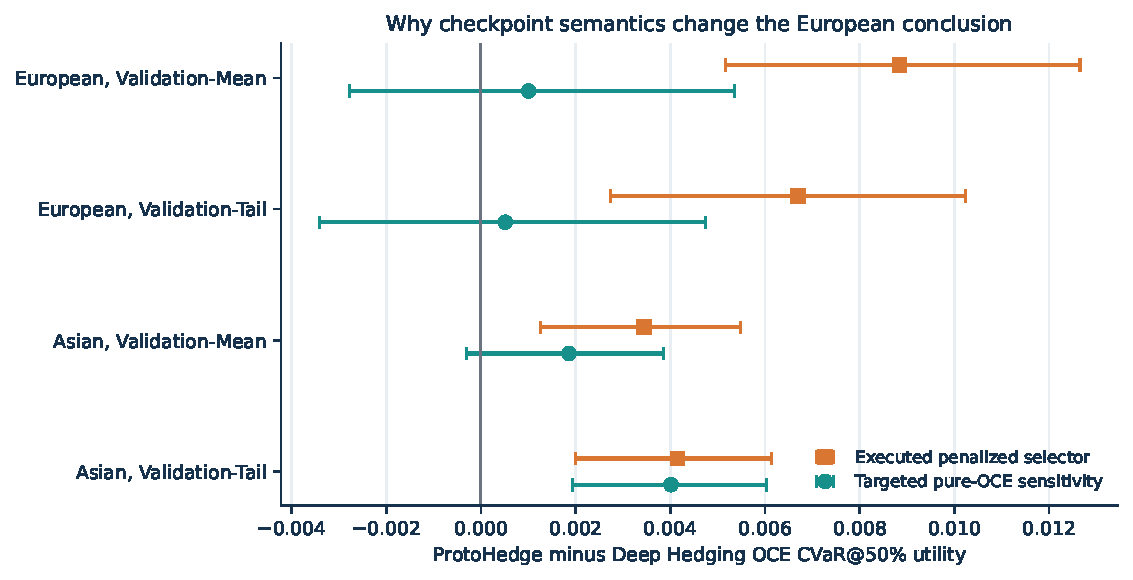
\includegraphics[width=0.86\textwidth]{checkpoint_sensitivity_comparison.pdf}
\caption{Executed diagnostic-penalized estimates and targeted pure-OCE
sensitivity estimates. The European superiority interpretation does not
survive the checkpoint audit; the Asian tail result changes little.}
\label{fig:checkpoint-change}
\end{figure*}

The Asian changes are smaller. Validation-Mean falls from $+0.003449$ to
$+0.001859$, and its revised interval narrowly crosses zero. Validation-Tail
changes from $+0.004151$ to $+0.004015$, a 3.3\% reduction, and its interval
remains positive. The asymmetric impact follows the audit incidence: 11
European DH fits but only one Asian DH fit selected initialization.

This audit prevents a stronger but unreliable narrative. The result is not
that the historical study failed. It is that European historical near parity
is the finding most consistent with both the corrected benchmark and the
original synthetic study.

\subsection{Conservative PH--DH Panel Results}

Table~\ref{tab:primary-historical} and Fig.~\ref{fig:primary-historical} report
the targeted sensitivity. The European Validation-Mean estimate is $+0.001009$
with interval $[-0.002777,0.005364]$; Validation-Tail is $+0.000514$ with
$[-0.003418,0.004734]$. Neither supports a detectable difference.

For Asian calls, Validation-Mean is $+0.001859$ with
$[-0.000309,0.003863]$, suggestive but not interval-separated from zero. The
Validation-Tail estimate is $+0.004015$ with
$[0.001925,0.006038]$, and every one of the 2,000 panel bootstrap draws is
positive. This is the one headline comparison whose interval excludes zero.

\begin{table}[t]
\centering
\footnotesize
\resizebox{\columnwidth}{!}{\begin{tabular}{llrrr}
\toprule
Liability & Selection & PH-DH & 95\% block interval & P(PH>DH) \\
\midrule
European & Validation-Mean & +0.001009 & [-0.002777, +0.005364] & 0.696 \\
European & Validation-Tail & +0.000514 & [-0.003418, +0.004734] & 0.602 \\
Asian & Validation-Mean & +0.001859 & [-0.000309, +0.003863] & 0.961 \\
Asian & Validation-Tail & +0.004015 & [+0.001925, +0.006038] & 1.000 \\
\bottomrule
\end{tabular}
}
\caption{Conservative historical PH--DH differences in frozen-threshold OCE
CVaR@50\% utility. Positive values favor the validation-selected expanded PH
family. These are hybrid targeted-sensitivity estimates, as defined in
Section~\ref{sec:audits}.}
\label{tab:primary-historical}
\end{table}

\begin{figure}[t]
\centering
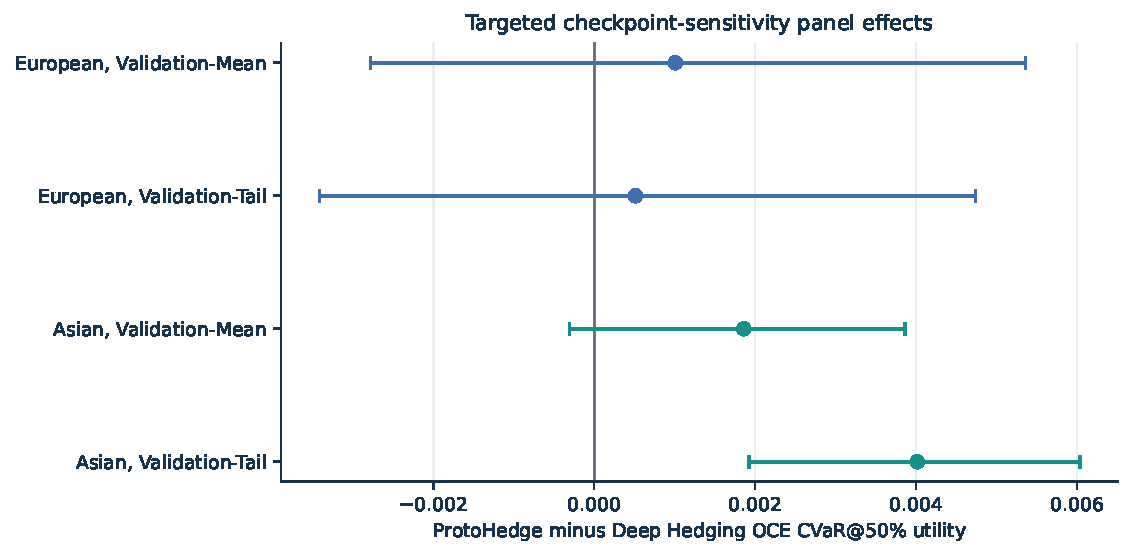
\includegraphics[width=\columnwidth]{audited_primary_cvar50.pdf}
\caption{Panel estimates and paired 95\% temporal-block intervals after the
targeted checkpoint sensitivity.}
\label{fig:primary-historical}
\end{figure}

Ticker-level results are heterogeneous. The Asian tail estimate is positive
for seven of ten tickers, with positive individual intervals for AAPL, NVDA,
TLT, and XLF and no ticker interval wholly below zero. European tail estimates
are positive for four of ten tickers; only TLT has an interval wholly above
zero. For Validation-Mean, Asian estimates are positive for seven tickers but
TLT is detectably negative, while European estimates are positive for seven
tickers with positive intervals for IWM and TLT. These patterns rule out a
uniform dominance claim and motivate the equal-ticker panel summary rather than
selective asset reporting.

\subsection{Comparison with Spot-Delta}

The Spot-Delta comparisons in Table~\ref{tab:spot-comparison} use the completed
historical PH checkpoints and are unaffected by replacement of DH checkpoints.
For European calls, both PH selections improve mean offset over Spot-Delta:
$+0.008849$ for Validation-Mean and $+0.005488$ for Validation-Tail, with
positive intervals. Their empirical CVaR@50\% differences are much smaller and
both intervals cross zero. Thus, the European PH family improves the center of
the premium-excluding offset distribution relative to this simple rule without
a supported 50\% lower-tail advantage.

For Asian calls, both selection rules have positive intervals for both mean
offset and empirical CVaR@50\%. Validation-Tail improves mean by $0.002795$ and
empirical CVaR@50\% by $0.005830$; Validation-Mean improves them by $0.004647$
and $0.005139$. This reinforces the path-dependent result against a transparent
baseline, although it remains tied to the selected expanded PH family and the
executed PH checkpoint semantics.

\begin{table*}[t]
\centering
\footnotesize
\resizebox{0.96\textwidth}{!}{\begin{tabular}{lllrr}
\toprule
Liability & Selection & Metric & PH-Spot Delta & 95\% block interval \\
\midrule
Asian & Validation-Mean & Empirical CVaR@50\% & +0.005139 & [+0.002159, +0.007676] \\
Asian & Validation-Mean & Mean offset & +0.004647 & [+0.002135, +0.007066] \\
Asian & Validation-Tail & Empirical CVaR@50\% & +0.005830 & [+0.002925, +0.008393] \\
Asian & Validation-Tail & Mean offset & +0.002795 & [+0.000271, +0.005291] \\
European & Validation-Mean & Empirical CVaR@50\% & +0.001114 & [-0.000986, +0.003142] \\
European & Validation-Mean & Mean offset & +0.008849 & [+0.007326, +0.010442] \\
European & Validation-Tail & Empirical CVaR@50\% & +0.000163 & [-0.001925, +0.002134] \\
European & Validation-Tail & Mean offset & +0.005488 & [+0.004086, +0.006858] \\
\bottomrule
\end{tabular}
}
\caption{Paired historical comparisons with Spot-Delta. Higher mean offset and
empirical CVaR@50\% are better; positive differences favor PH. These rows use
the completed historical PH protocol and are separate from the DH checkpoint
sensitivity.}
\label{tab:spot-comparison}
\end{table*}

\subsection{Saturation and Descriptive Performance}

Under the executed protocol, average DH test bound occupancy is approximately
39\% for both liabilities, and 69\% of paths touch a bound at least once when
pooled. The validation-selected PH rows have much lower average occupancy in
the descriptive table: approximately 4.2--5.3\% for European calls and
1.6--2.3\% for Asian calls. This supports the diagnostic statement that the PH
policies do not obtain their executed-protocol performance by occupying the
hard bounds more often than DH. It is not a causal explanation of performance,
and saturation is not used to define the conservative OCE result.

The full executed-protocol descriptive metrics are retained in
Appendix~\ref{app:descriptive}. They include mean offset, empirical CVaR@5\%,
RMSE, and occupancy for all six model labels. We do not use those raw model
levels to restore the pre-audit European superiority claim.

\subsection{SoftClip Sensitivity}

On the matched European SPY check, exact-TFP PH has OCE utility $-0.027027$,
historical-map PH has $-0.029020$, and DH has $-0.028771$. Exact PH minus DH is
$+0.001745$ with interval $[-0.009190,0.014586]$; historical PH minus DH is
$-0.000249$ with $[-0.011394,0.013623]$. Exact minus historical PH is
$+0.001993$ with $[-0.001693,0.006412]$. Every interval includes zero. This
small check finds no detectable reversal attributable to the map, while also
showing that the maps are not numerically interchangeable. The full panel
should therefore be described as a close architectural port with an audited
action-map sensitivity, not an exact numerical port.

\subsection{Prototype Usage and Example-Based Inspection}

We examine QQQ as a representative interpretability case because complete
artifacts are available for both liabilities. This analysis uses the PH models
selected under the completed historical protocol and is descriptive, not the
basis for selecting a performance result.

Let $\bar\alpha_k$ be mean assignment mass over test paths and times. Two
effective-library sizes are
\begin{equation}
K_{\mathrm{ent}}=\exp\left(-\sum_k\bar\alpha_k\log\bar\alpha_k\right),
\qquad
K_{\mathrm{inv}}=\left(\sum_k\bar\alpha_k^2\right)^{-1}.
\end{equation}
Both equal $K$ under uniform use and approach one under concentration.

\begin{table}[t]
\centering
\footnotesize
\resizebox{\columnwidth}{!}{\begin{tabular}{lrrrrr}
\toprule
Liability & Nominal K & Top-1 mass & Top-3 mass & Top-5 mass & Entropy effective K \\
\midrule
European & 10 & 0.244 & 0.582 & 0.831 & 7.31 \\
Asian & 50 & 0.585 & 0.696 & 0.738 & 14.03 \\
\bottomrule
\end{tabular}
}
\caption{Mean prototype concentration for the selected QQQ policies across
three seeds. The Asian averages have substantial cross-seed variability and
should not be interpreted as a stable single-policy sparsity estimate.}
\label{tab:interpretability}
\end{table}

For European QQQ, the nominal $K=10$ model assigns 24.4\% of mass to the most
used prototype, 58.2\% to the top three, and 83.1\% to the top five; its entropy
effective size is 7.31. The nominal $K=50$ Asian selection has mean top-one
mass 58.5\%, top-ten mass 80.7\%, and entropy effective size 14.03. However,
the Asian standard deviations are large (0.439 for top-one mass and 20.68 for
entropy effective size), revealing strong seed dependence that the mean alone
would obscure.

The dominant European prototype changes across return, volatility, and
drawdown terciles: P9 dominates down and middle returns, P2 dominates up
returns, P5 dominates low volatility, and P2 dominates middle/high volatility.
By contrast, Asian P39 is dominant in every reported bucket, with weight
ranging from 0.672 in high volatility to 0.938 in low volatility. Therefore the
European case exhibits prototype-identity switching, while the Asian case
shows strong concentration with regime-dependent mass but not a changing top
prototype.

The archived nearest-state records connect dominant anchors to concrete test
episodes, dates, contract identifiers, inventories, and normalized prices. This
supports exact example retrieval. It does not establish that users will find
the examples sufficient for every governance task, nor that the prototype
identity is stable under retraining.

\section{Discussion}

\subsection{Relation to the Original ProtoHedge Result}

The original PH paper found a small DH advantage in both synthetic worlds.
Our frozen-source experiments recover that direction. The checkpoint-corrected
historical European result is also near zero. From a validation perspective,
this is arguably more coherent than the initial large historical superiority:
the same prototype bottleneck that costs little utility in simulation also
costs no detectable utility on the ten-ticker terminal-call panel.

The Asian tail result is different. It is not a reproduction of either
synthetic world; it is an extension to a payoff that depends on the path. The
policy observes running-average moneyness, so PH and DH receive payoff-sufficient
information. The positive tail-selected panel estimate suggests that the
prototype bottleneck may regularize decisions usefully in this setting. The
result remains a family-level, validation-selected comparison, however, and
the present study cannot distinguish architectural regularization from the
benefit of the larger PH search budget.

\subsection{What Is Good About the Result}

Four aspects are encouraging. First, the original-source synthetic ordering is
recovered under both environments, anchoring the empirical study to the metric
used in the original work. Second, the corrected historical protocol spans ten
underlyings and a genuinely held-out three-year test calendar. Third, European
near parity survives a conservative benchmark repair, which supports the basic
performance--interpretability premise without relying on an implausibly weak DH
checkpoint. Fourth, the Asian tail estimate is positive both against DH under
the targeted sensitivity and against Spot-Delta under direct block-bootstrap
comparison.

The audit itself is also a strength. Reporting the initial stronger claim would
have produced a simpler story, but the apparent European advantage was not
stable to a scientifically relevant checkpoint rule. Making that change
visible improves the reliability and reproducibility of the final result.

\subsection{What Is Weaker Than Initially Expected}

The study no longer supports broad European PH superiority. The Asian
Validation-Mean interval also crosses zero. Ticker effects are heterogeneous,
and the Asian interpretability statistics vary substantially across seeds.
The full historical PH family includes extensions absent from the released
model, and its development budget is larger than DH's. Finally, the exact
SoftClip check covers one ticker, one liability, one seed, and one PH
configuration. These facts narrow the paper from a universal performance claim
to a careful empirical validation plus a promising path-dependent result.

\subsection{Implications for Reliable Sequential Decision Making}

The experiments illustrate a broader point. Reliability in sequential learning
is not only a property of the policy class. It also depends on the data unit,
state sufficiency, selection functional, benchmark budget, and uncertainty
estimator. Here, a single checkpoint convention altered the European
conclusion while leaving the raw test data untouched. Conversely, making the
Asian payoff state observable was necessary before any architectural
comparison could be meaningful.

Prototype policies offer one useful structural constraint: actions are routed
through a finite reference set that can be inspected and retrieved. A natural
next theoretical direction is to characterize when such a bottleneck improves
robustness under regime shift or limited data. Possible questions include
generalization bounds that depend on effective prototype usage rather than
nominal $K$, stability guarantees for prototype assignments under distribution
shift, and risk-sensitive regret bounds for prototype-constrained policies.
These questions go beyond the empirical claims of this paper but follow
directly from the observed near-parity and path-dependent behavior.

\section{Limitations and Threats to Validity}
\label{sec:limitations}

\textbf{Expanded PH family and unequal tuning.} PH searches 16 configurations
per seed and DH uses one fixed architecture. The experiment validates the
expanded PH family against the paper-style benchmark, not against a
hyperparameter-matched DH family. Twenty-five of 40 headline PH selections use
at least one extension.

\textbf{Hybrid checkpoint sensitivity.} The pure-OCE rerun is targeted at the
12 identified initialized DH fits and their matched selected PH candidates.
It is not a complete rerun of every epoch and every PH configuration under one
uniform new selector. We therefore report both executed and sensitivity
results and avoid calling the latter a definitive protocol replacement.

\textbf{Action-map scope.} The ten-ticker run uses the historical smooth map;
the exact TFP formula is tested only on one European SPY seed. The interval is
wide enough that a modest effect cannot be excluded.

\textbf{Premium and execution.} The outcome excludes the liability premium and
is not economic P\&L. Option prices are daily midquotes, and costs are stylized
rather than trade-level realized slippage. The selected listed option's vendor
delta is only a proxy for the delta of the synthetic liability.

\textbf{Dependence.} Circular blocks address overlap within ticker, but the
panel resampling does not fully model synchronous cross-ticker market shocks.
The block length is fixed at the episode horizon, and no block-length
sensitivity is used in the headline table.

\textbf{Coverage and selection.} Ten liquid underlyings do not represent all
asset classes, liquidity regimes, strikes, maturities, or option styles. The
liabilities are at-the-money, the horizon is fixed, and the validation and test
calendars contain specific market regimes. Two PH selection objectives create
related comparisons, and intervals are not multiplicity-adjusted.

\textbf{Synthetic reproducibility.} The original Black--Scholes zero-drift
prototype artifact is missing, the original test clone seed was not recorded,
and neural optimization is stochastic. The notebook-faithful run is close but
not numerically identical to the saved output.

\textbf{Training provenance.} The completed historical runner did not embed a
Git commit or full package freeze in each raw artifact. The archive records
this gap honestly: source and input files were checksummed at archive time, and
the locked cloud requirements are retained, but archive-time package versions
are not relabeled as training-time versions.

\textbf{Interpretability.} Equation~\eqref{eq:proto-action} makes the reported
weights faithful to action generation, but concentration and nearest examples
do not establish causal economic explanations, user usefulness, or retraining
stability.

\section{Reproducibility and Artifact Integrity}

The completed historical run contains 20 ticker--liability tasks and 4,025 raw
files totaling approximately 132 MB. SHA-256 manifests cover raw outputs, 53
panel inputs totaling approximately 136 MB, and 73 archive-time source files.
The synthetic directories separately retain source snapshots, environments,
protocol JSON files, training histories, model artifacts, test paths, and
checksums. The SPY confirmation retains 23 checked artifacts, and the
notebook-faithful Black--Scholes confirmation retains 16.

For this manuscript, a deterministic generator copies 43 compact source files
into a paper-facing archive, records their original paths and hashes, and
creates every CSV, LaTeX table, PDF figure, PNG preview, and a locked numerical
results ledger. Generated assets have a second checksum manifest. The generator
records Git HEAD \texttt{47c80a2b210d}, Python 3.12.2, NumPy 1.26.4, pandas
2.2.3, and Matplotlib 3.9.2 for the paper-asset build. These versions describe
asset generation, not the historical GPU training environment.

The intended reproduction commands are
\begin{verbatim}
cd paper/final_manuscript
python generate_assets.py
latexmk -pdf \
  protohedge_historical_validation.tex
\end{verbatim}
All manuscript numbers should be edited through the source data or generator,
not by changing the rendered tables manually.

\section{Conclusion}

We evaluated whether ProtoHedge's interpretable action bottleneck survives the
transition from stylized simulation to historical option paths. Frozen-source
synthetic experiments reproduce the original direction: PH is slightly below
DH in both Black--Scholes and stochastic-volatility environments. A corrected
ten-underlying historical panel then shows European near parity after a
targeted checkpoint repair, aligning the empirical result with that synthetic
premise. For arithmetic-average Asian liabilities, the tail-selected expanded
PH family retains a positive OCE CVaR@50\% panel interval and improves both mean
and empirical CVaR@50\% relative to Spot-Delta.

The most important methodological finding is that checkpoint semantics matter.
The initially stronger European result shrank by roughly 90\% after replacing
initialized DH selections under pure validation OCE. The final paper is
stronger for reporting that correction. The evidence supports PH as an
inspectable, competitive historical hedge and identifies path-dependent tail
risk as a promising setting, while leaving universal superiority, matched
model-family tuning, and full exact-map confirmation to future work.

\appendices

\section{Locked Historical Protocol}
\label{app:protocol}

Table~\ref{tab:protocol-full} lists the principal locked values. A machine-
readable JSON record is included in the artifact archive.

\begin{table*}[h]
\centering
\small
\begin{tabular}{lp{0.67\columnwidth}}
\toprule
Component & Locked value \\
\midrule
Underlyings & AAPL, IWM, NVDA, QQQ, SPY, TLT, XLE, XLF, XLK, XLV \\
Liabilities & European and arithmetic-average Asian ATM short calls \\
Episode timing & 20 decisions, 21 observations \\
Train / validation / test & 2005--2018 / 2019--2021 / 2022--2024 \\
Boundary embargo & 20 observations \\
Training seeds & 1234, 2345, 3456 \\
Epochs / learning rate & 800 / 0.001 \\
DH architecture & width 20, depth 3, Softplus \\
Prototype counts & 10, 25, 50, 100 \\
Prototype sources & Deep Hedging and Spot-Delta \\
Similarity variants & unweighted and hand-weighted \\
Trade / position bounds & [-1,1] per instrument \\
Bootstrap & 2000 paired circular-block draws; block 20 \\
\bottomrule
\end{tabular}

\caption{Locked historical protocol. A null batch override means the runner's
implementation default was retained rather than retroactively assigning a
batch size.}
\label{tab:protocol-full}
\end{table*}

\section{Original Executed-Protocol Descriptives}
\label{app:descriptive}

Table~\ref{tab:descriptive-full} reports model levels from the completed run.
These values are useful for scale, friction, and boundary diagnostics. They are
not substituted for the targeted PH--DH OCE sensitivity in the headline claim.

\begin{table*}[h]
\centering
\footnotesize
\resizebox{0.94\textwidth}{!}{\begin{tabular}{llrrrr}
\toprule
Liability & Model & Mean offset & CVaR@5\% & RMSE & Bound occ. \\
\midrule
European & Unhedged & -0.031696 & -0.137725 & 0.051082 & 0.0\% \\
European & Spot-Delta & -0.030281 & -0.070542 & 0.033481 & 0.0\% \\
European & Spot-Delta Band & -0.029875 & -0.073046 & 0.033661 & 0.0\% \\
European & Deep Hedging & -0.023872 & -0.113276 & 0.041646 & 39.0\% \\
European & ProtoHedge (Validation-Mean) & -0.021432 & -0.094189 & 0.035060 & 5.3\% \\
European & ProtoHedge (Validation-Tail) & -0.024793 & -0.084112 & 0.033853 & 4.2\% \\
Asian & Unhedged & -0.018544 & -0.082546 & 0.030284 & 0.0\% \\
Asian & Spot-Delta & -0.017129 & -0.065298 & 0.029230 & 0.0\% \\
Asian & Spot-Delta Band & -0.016724 & -0.066718 & 0.028730 & 0.0\% \\
Asian & Deep Hedging & -0.016210 & -0.082270 & 0.030993 & 39.3\% \\
Asian & ProtoHedge (Validation-Mean) & -0.012483 & -0.085456 & 0.029431 & 2.3\% \\
Asian & ProtoHedge (Validation-Tail) & -0.014334 & -0.077504 & 0.026745 & 1.6\% \\
\bottomrule
\end{tabular}
}
\caption{Equal-ticker averages under the originally executed historical
checkpoint protocol. CVaR@5\% is the empirical lower 5\% mean, not the OCE
CVaR@50\% training utility. Lower RMSE and occupancy are better.}
\label{tab:descriptive-full}
\end{table*}

\section{Per-Ticker Targeted Sensitivity}

Tables~\ref{tab:ticker-euro} and \ref{tab:ticker-asian} report every ticker;
Fig.~\ref{fig:ticker-effects} displays the same intervals. No assets are omitted
from panel conclusions.

\begin{table*}[h]
\centering
\footnotesize
\resizebox{0.92\textwidth}{!}{\begin{tabular}{lrrrr}
\toprule
Ticker & Mean sel. & 95\% interval & Tail sel. & 95\% interval \\
\midrule
AAPL & +0.000790 & [-0.0129, +0.0152] & +0.004558 & [-0.0092, +0.0204] \\
IWM & +0.009644 & [+0.0033, +0.0166] & +0.001921 & [-0.0059, +0.0104] \\
NVDA & -0.014811 & [-0.0407, +0.0167] & -0.012413 & [-0.0344, +0.0139] \\
QQQ & -0.001108 & [-0.0096, +0.0086] & -0.000598 & [-0.0160, +0.0166] \\
SPY & +0.000893 & [-0.0083, +0.0109] & -0.001670 & [-0.0116, +0.0103] \\
TLT & +0.009319 & [+0.0028, +0.0164] & +0.017408 & [+0.0083, +0.0267] \\
XLE & +0.000701 & [-0.0079, +0.0105] & -0.000484 & [-0.0069, +0.0069] \\
XLF & +0.004714 & [-0.0008, +0.0109] & -0.001828 & [-0.0072, +0.0036] \\
XLK & -0.000783 & [-0.0117, +0.0110] & +0.001573 & [-0.0053, +0.0092] \\
XLV & +0.000725 & [-0.0069, +0.0082] & -0.003326 & [-0.0103, +0.0042] \\
\bottomrule
\end{tabular}
}
\caption{European PH--DH frozen-threshold OCE CVaR@50\% differences under the
hybrid targeted checkpoint sensitivity.}
\label{tab:ticker-euro}
\end{table*}

\begin{table*}[h]
\centering
\footnotesize
\resizebox{0.92\textwidth}{!}{\begin{tabular}{lrrrr}
\toprule
Ticker & Mean sel. & 95\% interval & Tail sel. & 95\% interval \\
\midrule
AAPL & +0.001200 & [-0.0028, +0.0056] & +0.006108 & [+0.0016, +0.0110] \\
IWM & +0.007285 & [+0.0011, +0.0129] & +0.004657 & [-0.0030, +0.0126] \\
NVDA & +0.014533 & [+0.0062, +0.0220] & +0.014533 & [+0.0067, +0.0220] \\
QQQ & +0.003307 & [-0.0019, +0.0082] & +0.003307 & [-0.0022, +0.0083] \\
SPY & +0.001395 & [-0.0032, +0.0067] & -0.000483 & [-0.0052, +0.0050] \\
TLT & -0.008643 & [-0.0132, -0.0039] & +0.008796 & [+0.0053, +0.0127] \\
XLE & -0.002502 & [-0.0141, +0.0076] & -0.001143 & [-0.0104, +0.0082] \\
XLF & +0.003464 & [+0.0002, +0.0065] & +0.003464 & [+0.0003, +0.0068] \\
XLK & -0.002604 & [-0.0123, +0.0070] & -0.002802 & [-0.0122, +0.0067] \\
XLV & +0.001158 & [-0.0039, +0.0060] & +0.003715 & [-0.0009, +0.0083] \\
\bottomrule
\end{tabular}
}
\caption{Asian PH--DH frozen-threshold OCE CVaR@50\% differences under the
hybrid targeted checkpoint sensitivity.}
\label{tab:ticker-asian}
\end{table*}

\begin{figure*}[h]
\centering
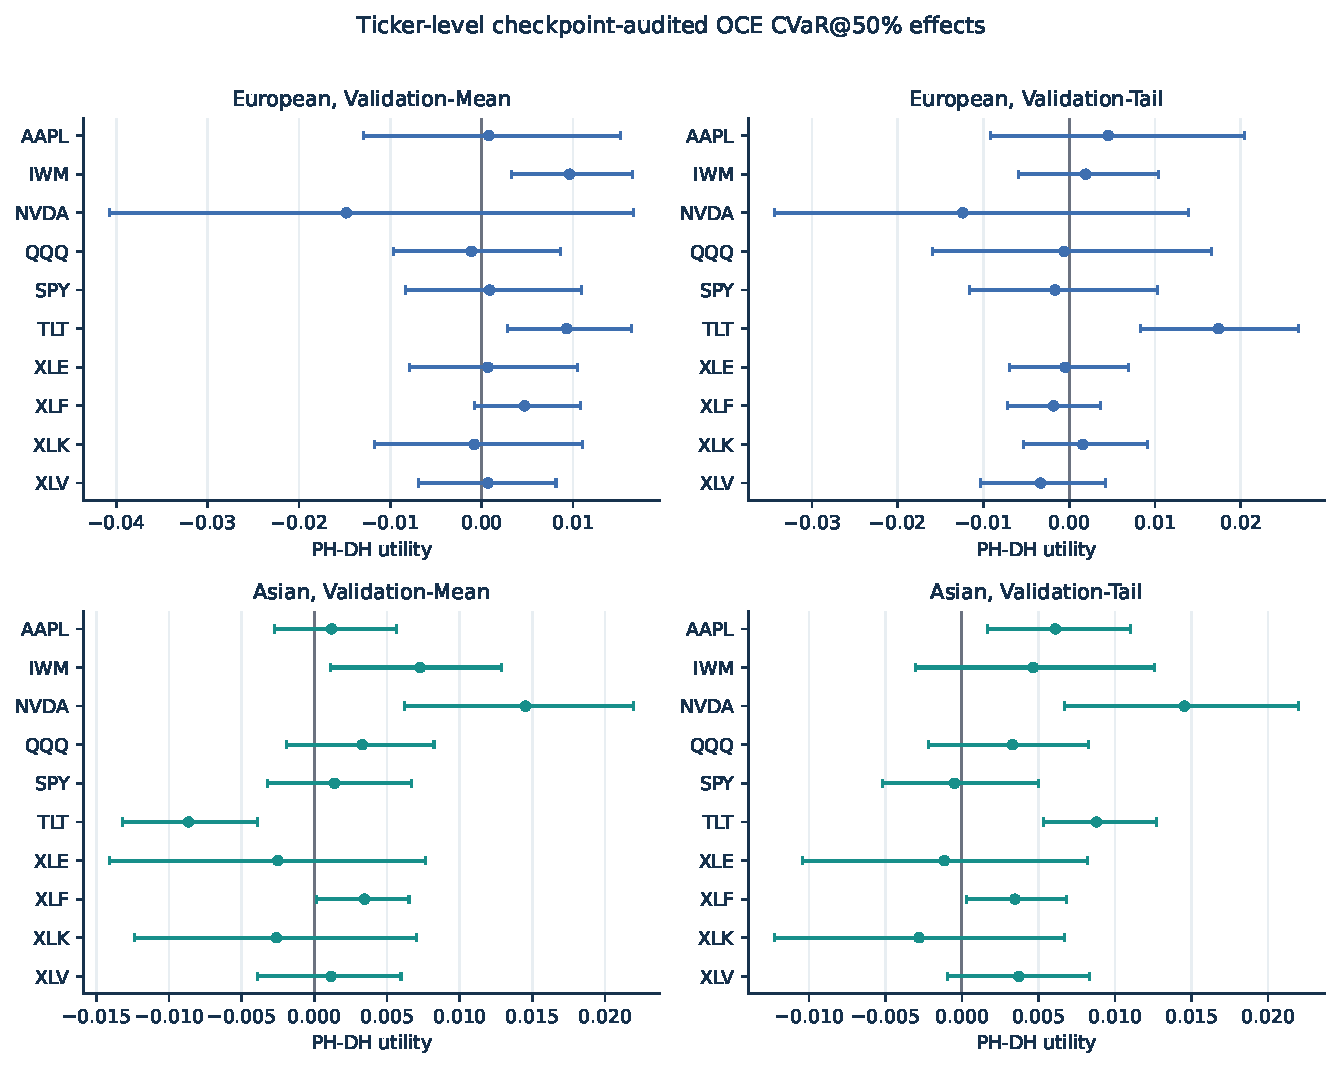
\includegraphics[width=0.90\textwidth]{audited_per_ticker_cvar50.pdf}
\caption{Ticker-level central estimates and paired temporal-block intervals.
Heterogeneity is visible for both liabilities and selection objectives.}
\label{fig:ticker-effects}
\end{figure*}

\section{Checkpoint and Family-Scope Diagnostics}

\begin{table*}[h]
\centering
\footnotesize
\resizebox{0.93\textwidth}{!}{\begin{tabular}{lrrrrrr}
\toprule
Liability & Fits & Epoch -1 & Fraction & Median trained epoch & Test bound occ. & Paths touching bound \\
\midrule
All & 60 & 12 & 20.0\% & 38.0 & 39.2\% & 69.1\% \\
Asian & 30 & 1 & 3.3\% & 70.0 & 39.3\% & 71.7\% \\
European & 30 & 11 & 36.7\% & 16.0 & 39.0\% & 66.5\% \\
\bottomrule
\end{tabular}
}
\caption{Deep Hedging checkpoint and saturation audit from the completed run.
Epoch $-1$ denotes the initialized checkpoint. ``Paths touching bound'' is a
path-level diagnostic and can be high even when average occupancy is lower.}
\label{tab:dh-audit}
\end{table*}

\begin{table}[h]
\centering
\footnotesize
\resizebox{\columnwidth}{!}{\begin{tabular}{lrrr}
\toprule
Liability & Released-paper-like & Uses extension & Total selections \\
\midrule
European & 5 & 15 & 20 \\
Asian & 10 & 10 & 20 \\
All & 15 & 25 & 40 \\
\bottomrule
\end{tabular}
}
\caption{Scope of the selected historical PH family. Each ticker contributes a
mean and tail selection per liability.}
\label{tab:family-scope}
\end{table}

\section{Black--Scholes Alignment Detail}

\begin{table}[h]
\centering
\footnotesize
\resizebox{\columnwidth}{!}{\begin{tabular}{lrrr}
\toprule
Model & Reproduction & Saved notebook & Absolute error \\
\midrule
Deep Hedging & -0.058102 & -0.058166 & 0.000063 \\
ProtoHedge & -0.059013 & -0.058421 & 0.000592 \\
\bottomrule
\end{tabular}
}
\caption{Notebook-faithful Black--Scholes utility levels versus the values
stored in the released author notebook.}
\label{tab:bs-alignment}
\end{table}

\section{SoftClip Confirmation Detail}

\begin{table*}[h]
\centering
\footnotesize
\resizebox{0.96\textwidth}{!}{\begin{tabular}{lrrrrrr}
\toprule
Model & Epoch & OCE CVaR@50\% & Mean & Empirical CVaR@50\% & CVaR@5\% & Bound occ. \\
\midrule
Deep Hedging & 180 & -0.028771 & -0.014452 & -0.028549 & -0.093524 & 0.500 \\
ProtoHedge exact TFP & 532 & -0.027027 & -0.015661 & -0.025312 & -0.056798 & 0.170 \\
ProtoHedge historical & 356 & -0.029020 & -0.020097 & -0.028398 & -0.053125 & 0.073 \\
\bottomrule
\end{tabular}
}
\caption{European SPY, seed 2345, model-level metrics. These are a one-seed
implementation sensitivity and not panel inference.}
\label{tab:softclip-levels}
\end{table*}

\begin{table*}[h]
\centering
\footnotesize
\resizebox{0.92\textwidth}{!}{\begin{tabular}{lrrr}
\toprule
Contrast & Difference & 95\% block interval & P(>0) \\
\midrule
ProtoHedge exact TFP vs. Deep Hedging & +0.001745 & [-0.009190, +0.014586] & 0.589 \\
ProtoHedge historical vs. Deep Hedging & -0.000249 & [-0.011394, +0.013623] & 0.471 \\
ProtoHedge exact TFP vs. ProtoHedge historical & +0.001993 & [-0.001693, +0.006412] & 0.846 \\
\bottomrule
\end{tabular}
}
\caption{Paired temporal-block contrasts for the SoftClip sensitivity. All 95\%
intervals contain zero.}
\label{tab:softclip-contrasts}
\end{table*}

\begin{figure*}[h]
\centering
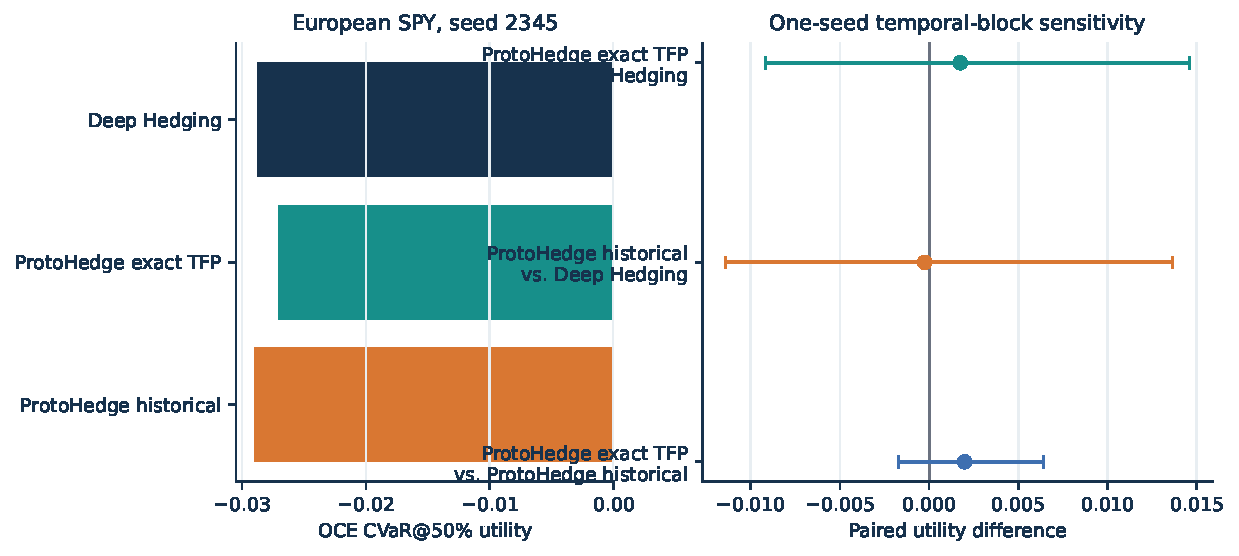
\includegraphics[width=0.84\textwidth]{spy_softclip_sensitivity.pdf}
\caption{Model levels and paired contrasts in the one-seed exact-SoftClip SPY
confirmation.}
\label{fig:softclip}
\end{figure*}

\section{Interpretability Detail}

\begin{figure}[h]
\centering
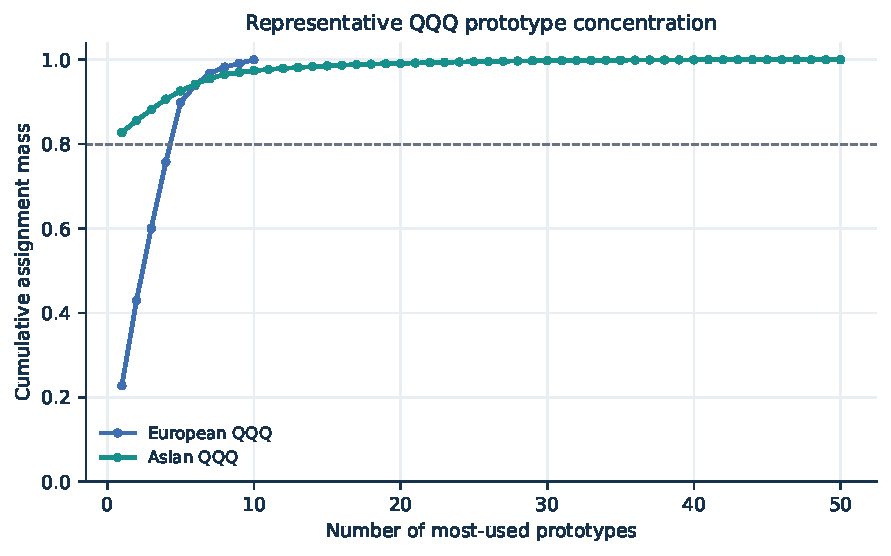
\includegraphics[width=\columnwidth]{qqq_prototype_concentration.pdf}
\caption{Cumulative mean prototype assignment mass for representative QQQ
policies. The three-seed Asian average hides substantial seed variability.}
\label{fig:prototype-concentration}
\end{figure}

\begin{table*}[h]
\centering
\footnotesize
\resizebox{0.90\textwidth}{!}{\begin{tabular}{llllr}
\toprule
Liability & Partition & Regime & Dominant prototype & Mean weight \\
\midrule
European & Drawdown & Deep & P2 & 0.293 \\
European & Drawdown & Middle & P2 & 0.260 \\
European & Drawdown & Mild & P9 & 0.291 \\
European & Return & Down & P9 & 0.316 \\
European & Return & Middle & P9 & 0.211 \\
European & Return & Up & P2 & 0.374 \\
European & Volatility & High & P2 & 0.249 \\
European & Volatility & Low & P5 & 0.232 \\
European & Volatility & Middle & P2 & 0.277 \\
Asian & Drawdown & Deep & P39 & 0.923 \\
Asian & Drawdown & Middle & P39 & 0.846 \\
Asian & Drawdown & Mild & P39 & 0.714 \\
Asian & Return & Down & P39 & 0.745 \\
Asian & Return & Middle & P39 & 0.894 \\
Asian & Return & Up & P39 & 0.844 \\
Asian & Volatility & High & P39 & 0.672 \\
Asian & Volatility & Low & P39 & 0.938 \\
Asian & Volatility & Middle & P39 & 0.872 \\
\bottomrule
\end{tabular}
}
\caption{Dominant QQQ prototype by return, volatility, and drawdown tercile for
the completed-protocol representative policies.}
\label{tab:regime-prototypes}
\end{table*}

\begin{table*}[h]
\centering
\scriptsize
\resizebox{0.99\textwidth}{!}{\begin{tabular}{lllrrrrrr}
\toprule
Liability & Proto. & Episode & Step & $h^S$ & $h^C$ & $S/S_0$ & $C/S_0$ & Asian state \\
\midrule
European & P1 & 2024-04-29 to 2024-05-28 & 6 & 0.686 & 0.007 & 1.017 & 0.024 & -- \\
European & P2 & 2023-05-25 to 2023-06-26 & 5 & 0.889 & -0.001 & 1.044 & 0.041 & -- \\
European & P5 & 2024-06-14 to 2024-07-16 & 2 & 0.571 & 0.003 & 1.013 & 0.019 & -- \\
European & P9 & 2024-05-29 to 2024-06-27 & 1 & 0.348 & 0.003 & 0.989 & 0.006 & -- \\
Asian & P20 & 2022-05-24 to 2022-06-23 & 14 & -0.018 & 0.009 & 0.961 & 0.010 & 1.044 \\
Asian & P27 & 2022-05-26 to 2022-06-27 & 11 & -0.125 & -0.154 & 0.920 & 0.006 & 1.012 \\
Asian & P36 & 2022-05-24 to 2022-06-23 & 14 & -0.018 & 0.009 & 0.961 & 0.010 & 1.044 \\
Asian & P39 & 2022-05-11 to 2022-06-09 & 5 & 0.013 & -0.137 & 0.998 & 0.041 & 1.020 \\
\bottomrule
\end{tabular}
}
\caption{Nearest rank-one historical state for selected dominant QQQ
prototypes. $h^S$ and $h^C$ are inventories; prices are normalized by initial
spot. The Asian state is running-average moneyness.}
\label{tab:nearest-states}
\end{table*}

\begin{figure*}[h]
\centering
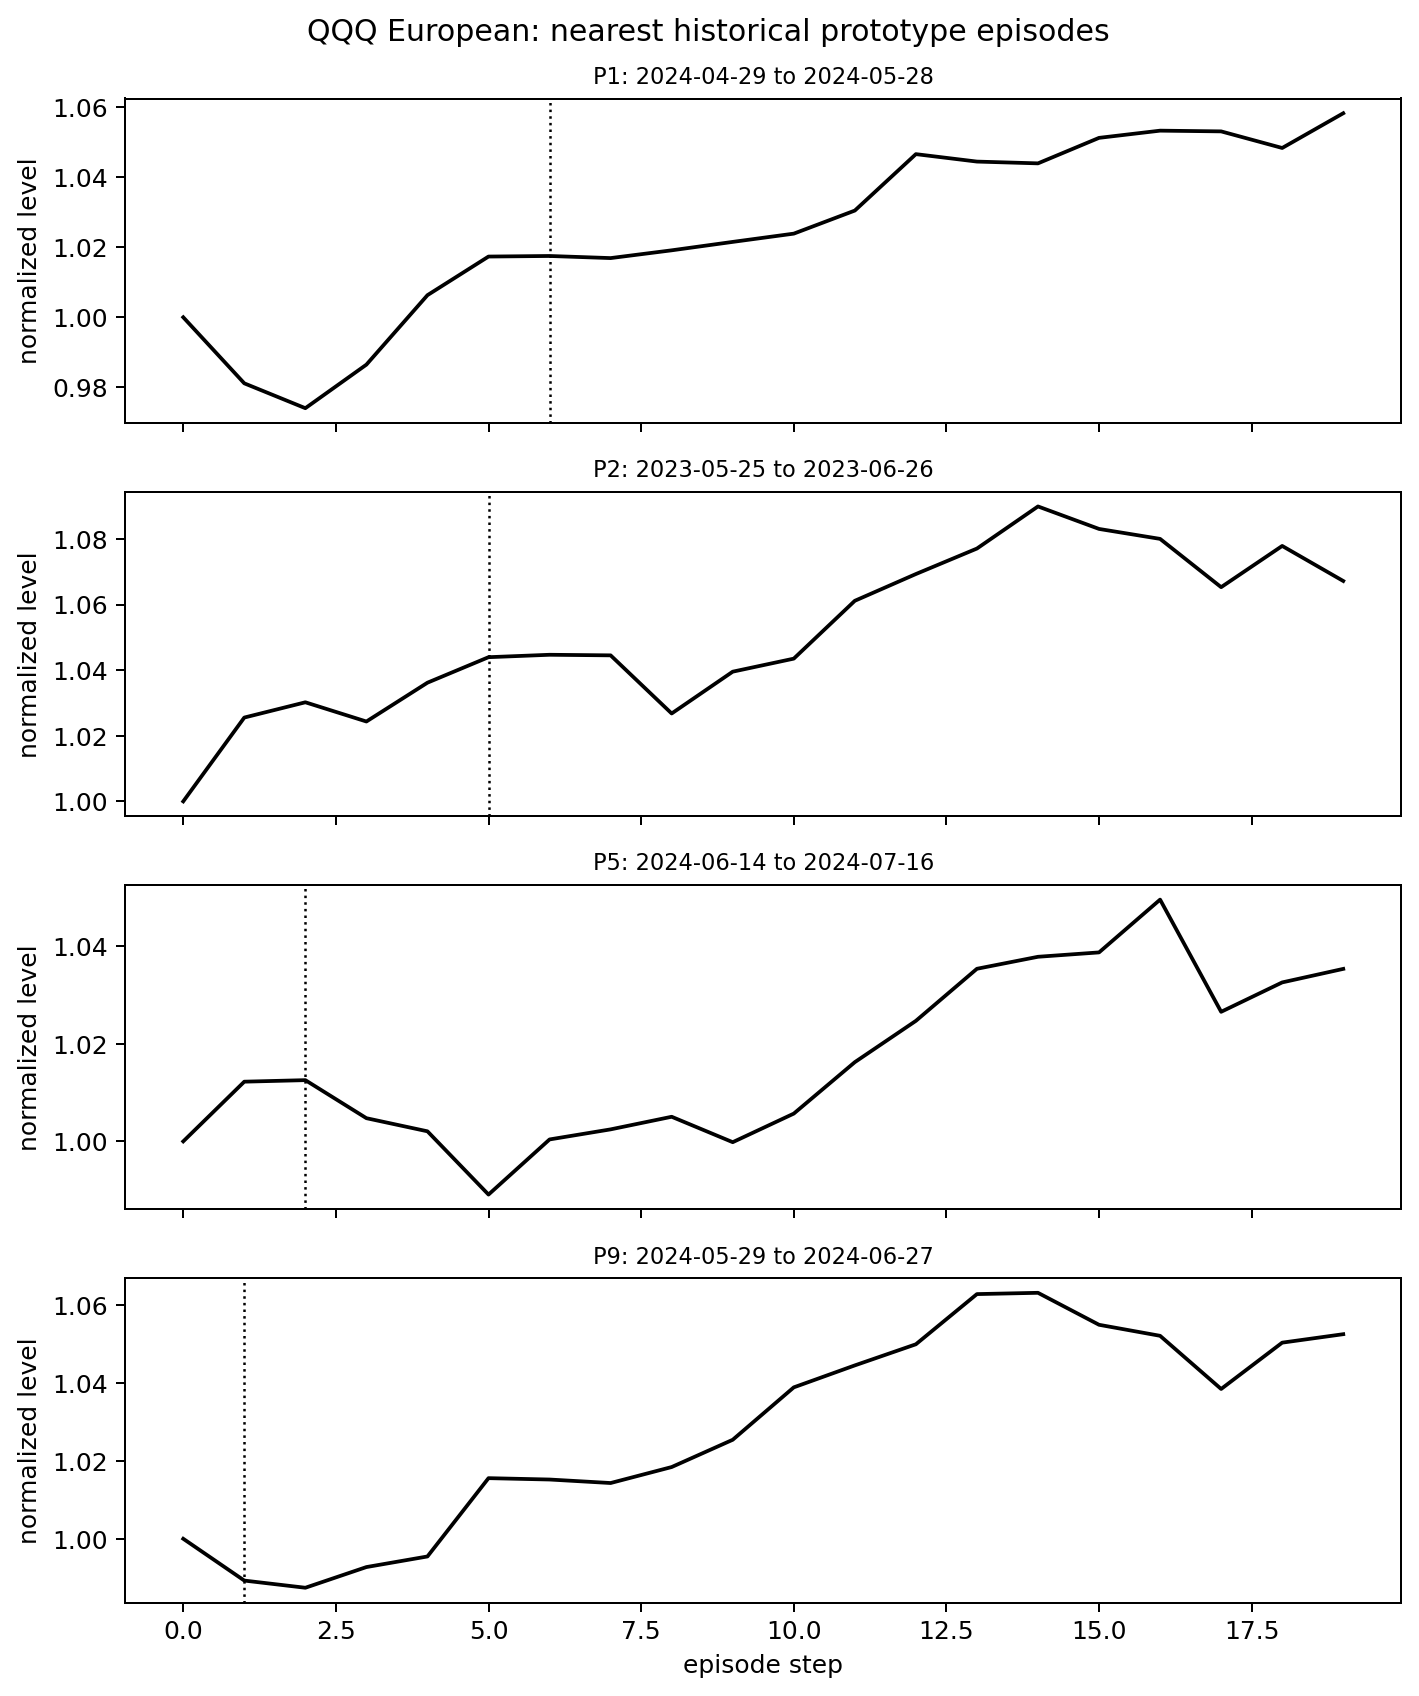
\includegraphics[width=0.90\textwidth]{qqq_european_nearest_episodes.png}
\caption{Retrieved European QQQ historical episodes nearest to selected
prototype states. This is an example-based inspection aid, not a performance
comparison.}
\label{fig:nearest-euro}
\end{figure*}

\begin{figure*}[h]
\centering
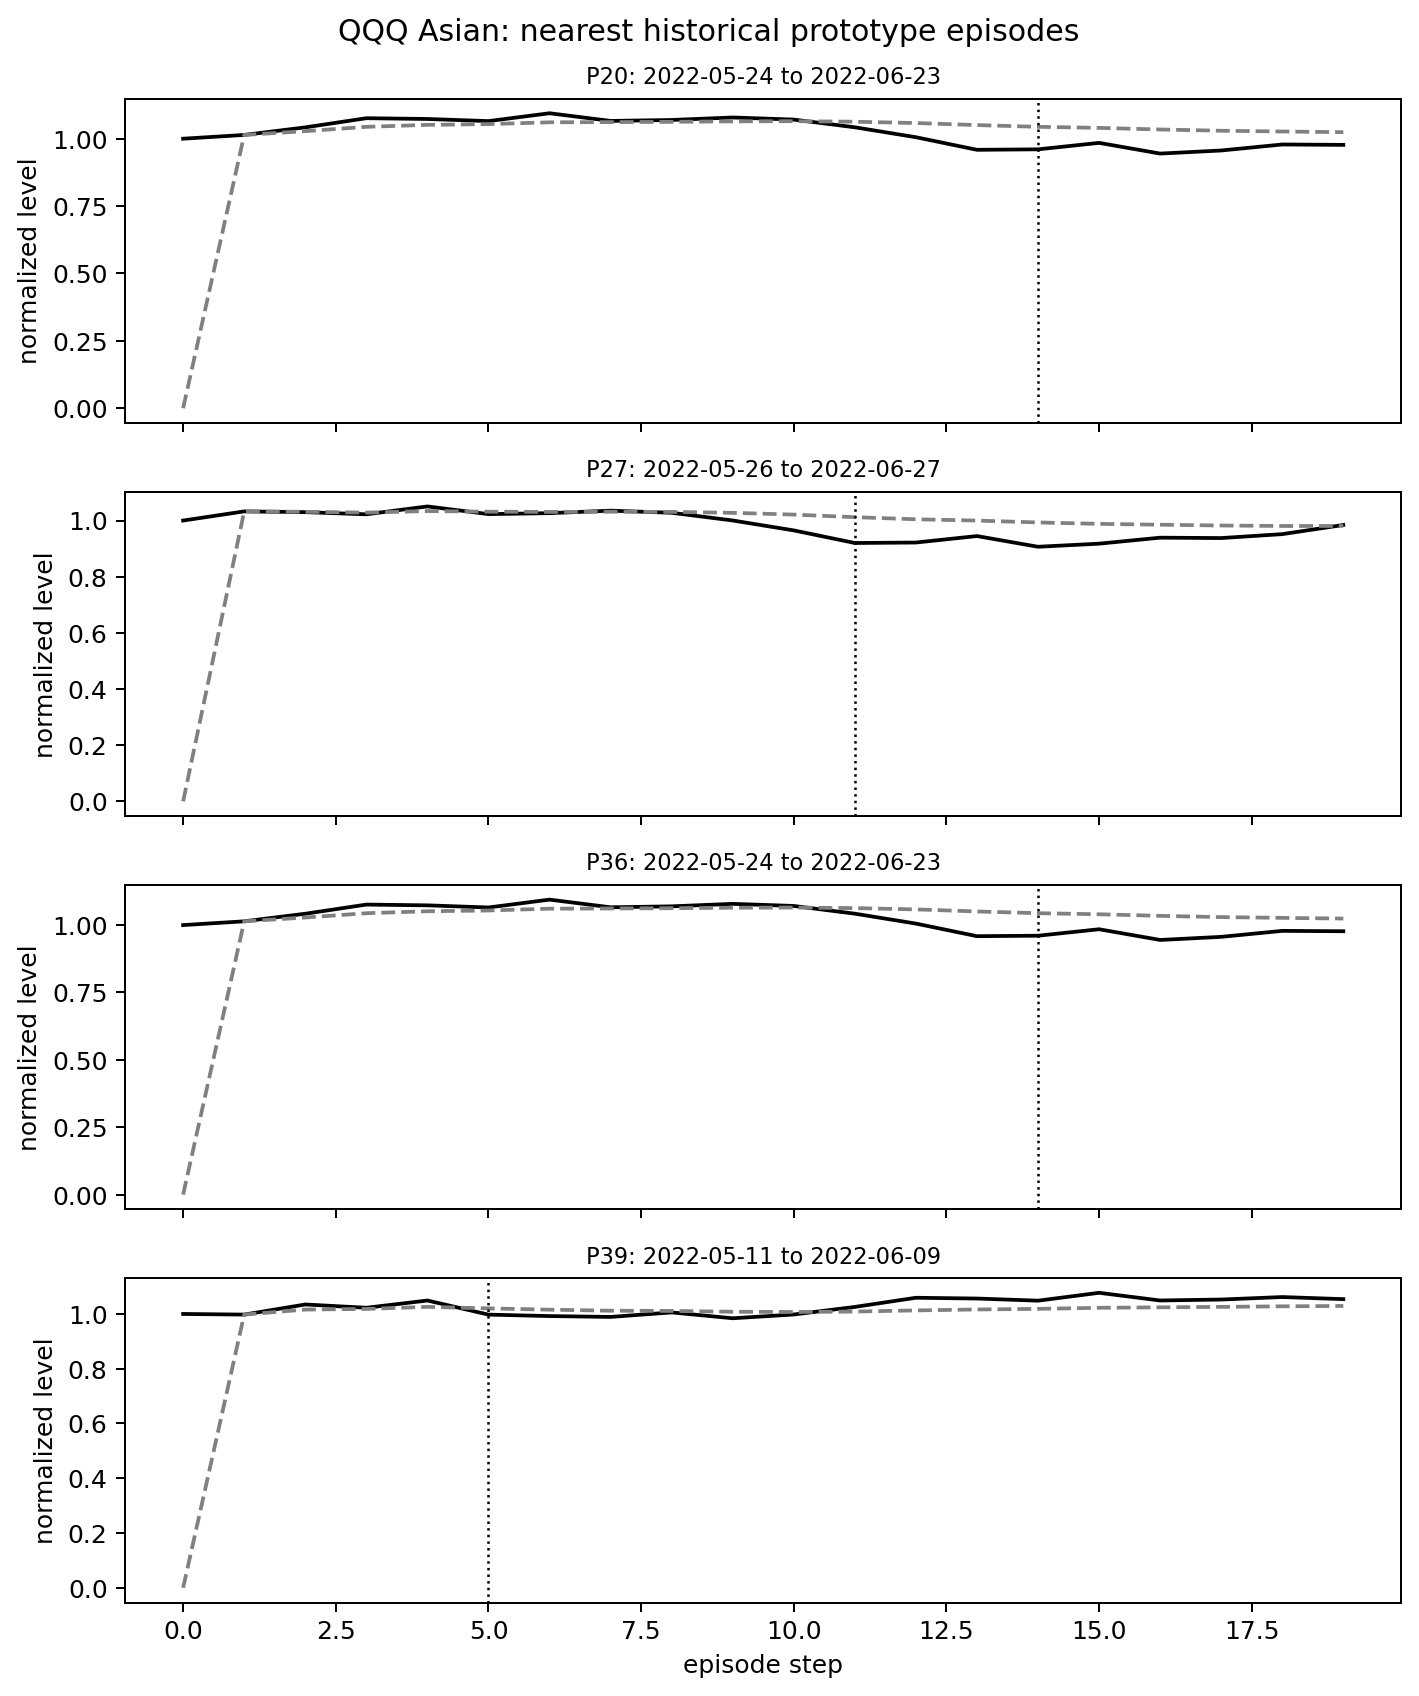
\includegraphics[width=0.90\textwidth]{qqq_asian_nearest_episodes.png}
\caption{Retrieved Asian QQQ historical episodes nearest to selected prototype
states.}
\label{fig:nearest-asian}
\end{figure*}

\bibliographystyle{IEEEtran}
\bibliography{references}

\end{document}
